\documentclass{article}
\usepackage[utf8]{inputenc}
\usepackage[a4paper, total={6in, 10in}]{geometry}
\usepackage{pgfplots}
\usepackage{array}
\usepackage{float}
\usepackage{graphicx}
\usepackage{amssymb}
\usepackage{amsmath}
\usepackage{parskip}
% \usepackage{biblatex}
\graphicspath{ {./images/} }

\usepackage{url}
\usepackage[colorlinks,allcolors=black]{hyperref}

\usepackage{blindtext}

\title{Exploring mathematics of rolling bridges \\
    \large Extended essay \\
    \vspace{12pt} Word count: 1}

\date{\today}
\author{Bartek Włodarczyk}


\pgfplotsset{compat=1.18}
\renewcommand{\arraystretch}{1.7}

\begin{document}

    \maketitle
    \newpage
    \tableofcontents
    \newpage
    
    \section{Research question}

    How can catenary curves be used in construction of non-circular "rolling" bridges?
    
    \section{Introduction}
    
        \begin{enumerate}
            \item My personal interest - I am interested in architecture and urban planning and this topic combines this with my passion for mathematics
            \item I have found this bridge in an internet video - as an interesting mathematical phenomena existing in real life
        \end{enumerate}

        \begin{figure}[H]
            \centering
            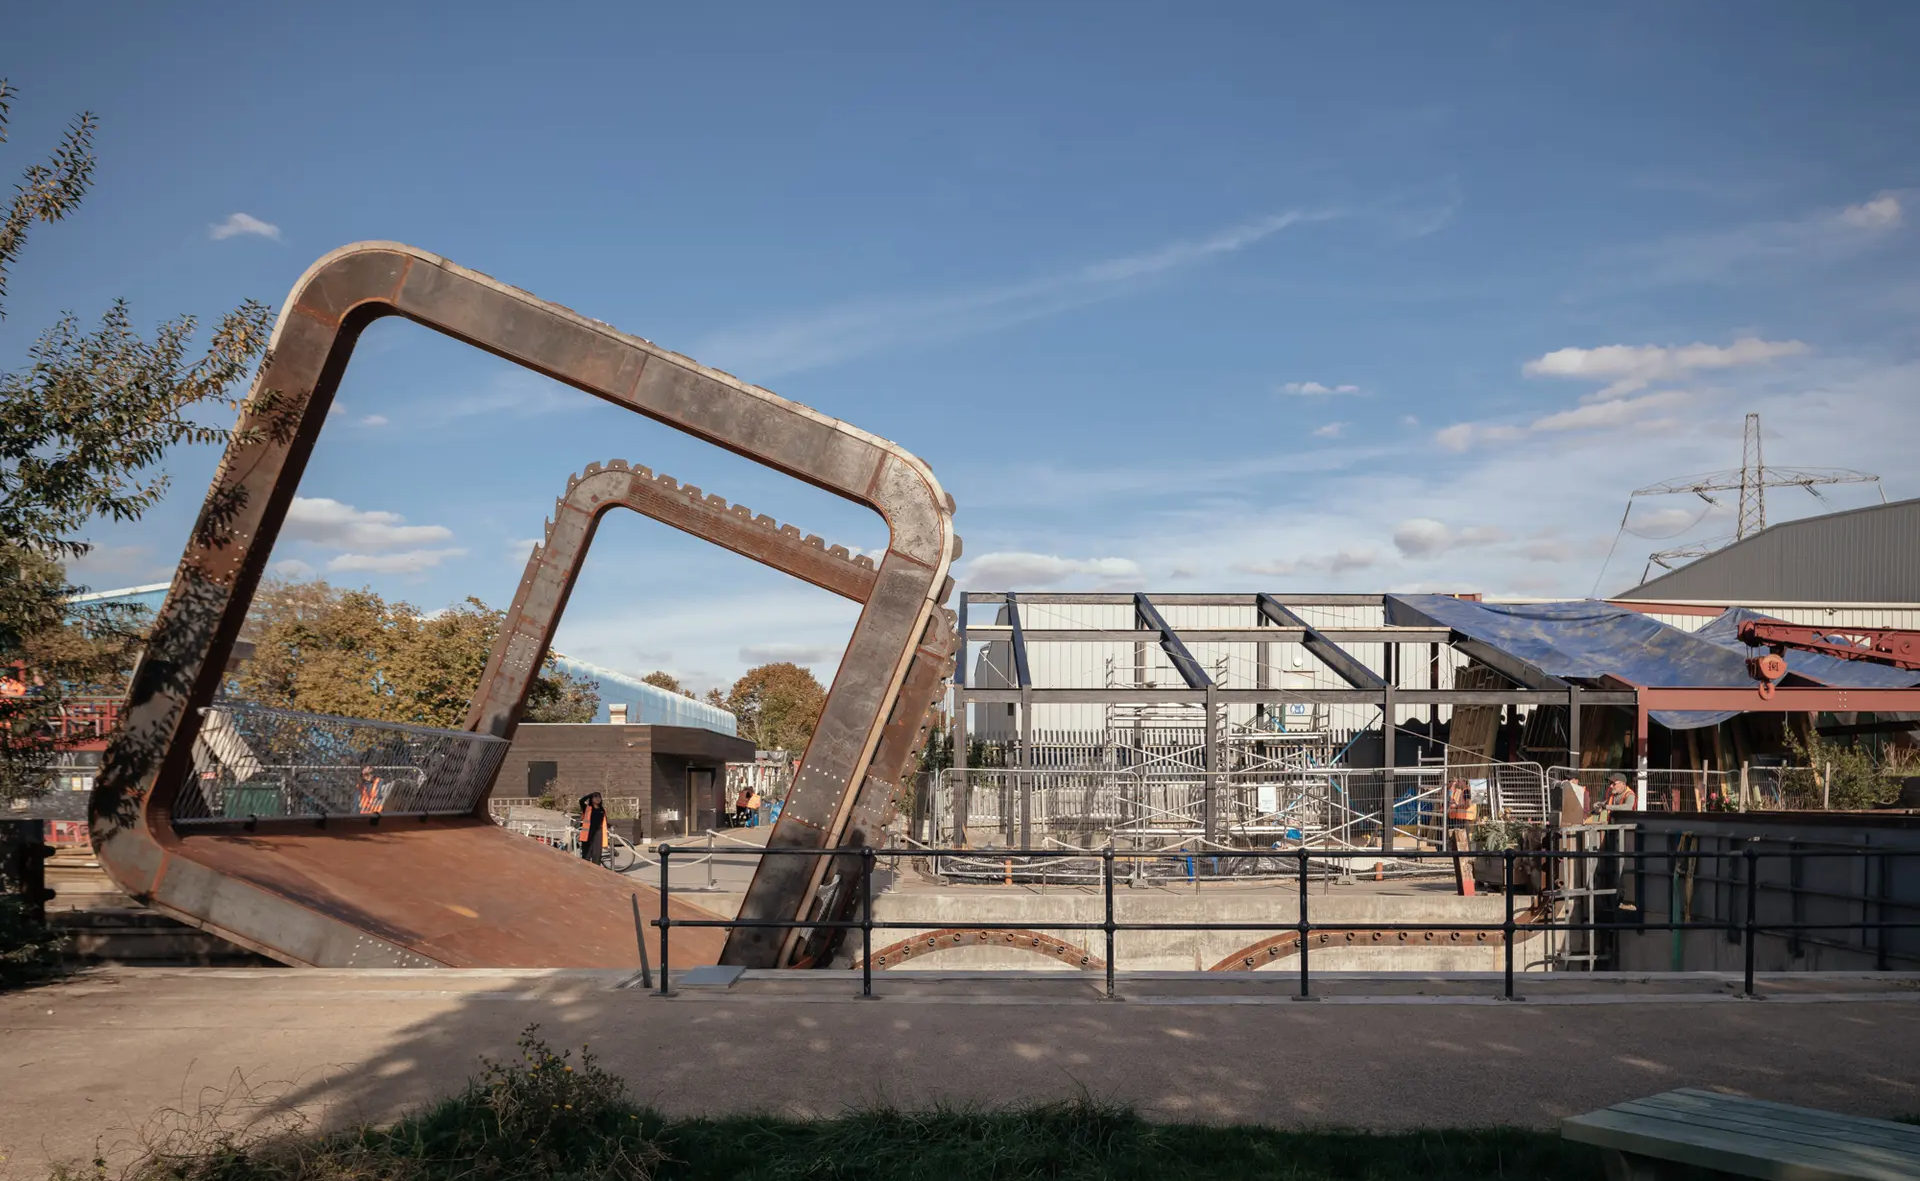
\includegraphics[width=0.75\linewidth]{images/bridge.png}
            \caption{Bridge photo \url{https://newatlas.com/architecture/cody-dock-rolling-bridge/}}
            \label{fig:enter-label}
        \end{figure}

    \section{References}

        \begin{enumerate}
            \item \url{https://community.wolfram.com/groups/-/m/t/2917199}
            \item \url{https://youtu.be/SsGEcLwjgEg}
            \item \url {https://youtu.be/xGxSTzaID3k}
        \end{enumerate}

    \newpage

    \section{Work plan}

        \begin{enumerate}
            \item square bridge \begin{enumerate}
                \item simple rolling square \begin{enumerate}
                    \item finding polar form - straight line times 4
                    \item finding relation between road and "wheel"
                    \item get y(t), then find road equation in y(x) form
                    \item catenary road = -cosh x
                \end{enumerate}
                \item rounded square \begin{enumerate}
                    \item why rounded - gears teeth
                    \item why rounded corners are hard - rolling on a circle, but centre of mass is outside of it
                    \item calculating road for the rounded square \begin{enumerate}
                        \item polar form of a rounded corner
                        \item symbolic solution \begin{itemize}
                            \item definite integration
                            \item elliptic integral of 2nd kind
                            \item cant get y(x)
                        \end{itemize}
                        \item numerical solution
                    \end{enumerate}
                    \item setting centre of mass to be at geometric centre (adding additional weight at the top of the bridge)
                    \item find location of gear teeth - roll the track around and trace intersection with bridge - inverse transformation of track around the bridge
                    \item calculating work needed to be done to roll the bridge - the centre of mass is actually 2inches below the geometric centre
                \end{enumerate}
            \end{enumerate}
            \item triangle bridge \begin{enumerate}
                \item normally cannot - too steep road and triangle crashes, but with rounded corners its possible
                \item the catenary curve is steeper, so more friction is needed
            \end{enumerate}
            \item polygonal bridge \begin{enumerate}
                \item pentagon and hexagon
            \end{enumerate}
            \item conclusion
        \end{enumerate}
    
    % \section{Conclusion}
    
    %     \subsection{Reflections}    
    
    %     \subsection{Limitations}
    
    %         How to improve, etc.
        
\end{document}
